\documentclass[../thesis.tex]{subfiles}
\begin{document}

\chapter{parametric study}
\label{chp: para_stud}
Within the parametric study the three different reactor geometries are simulated under different flow conditions. These different conditions, as shown in \autoref{tab: cases}, lead to different front shapes. Two of these front shapes can be seen in \autoref{fig: shape_examp}.
\begin{figure}[htb]
	\centering
	\subfloat[\centering front shape for h0.6mm Pe2050 Sc12000]{{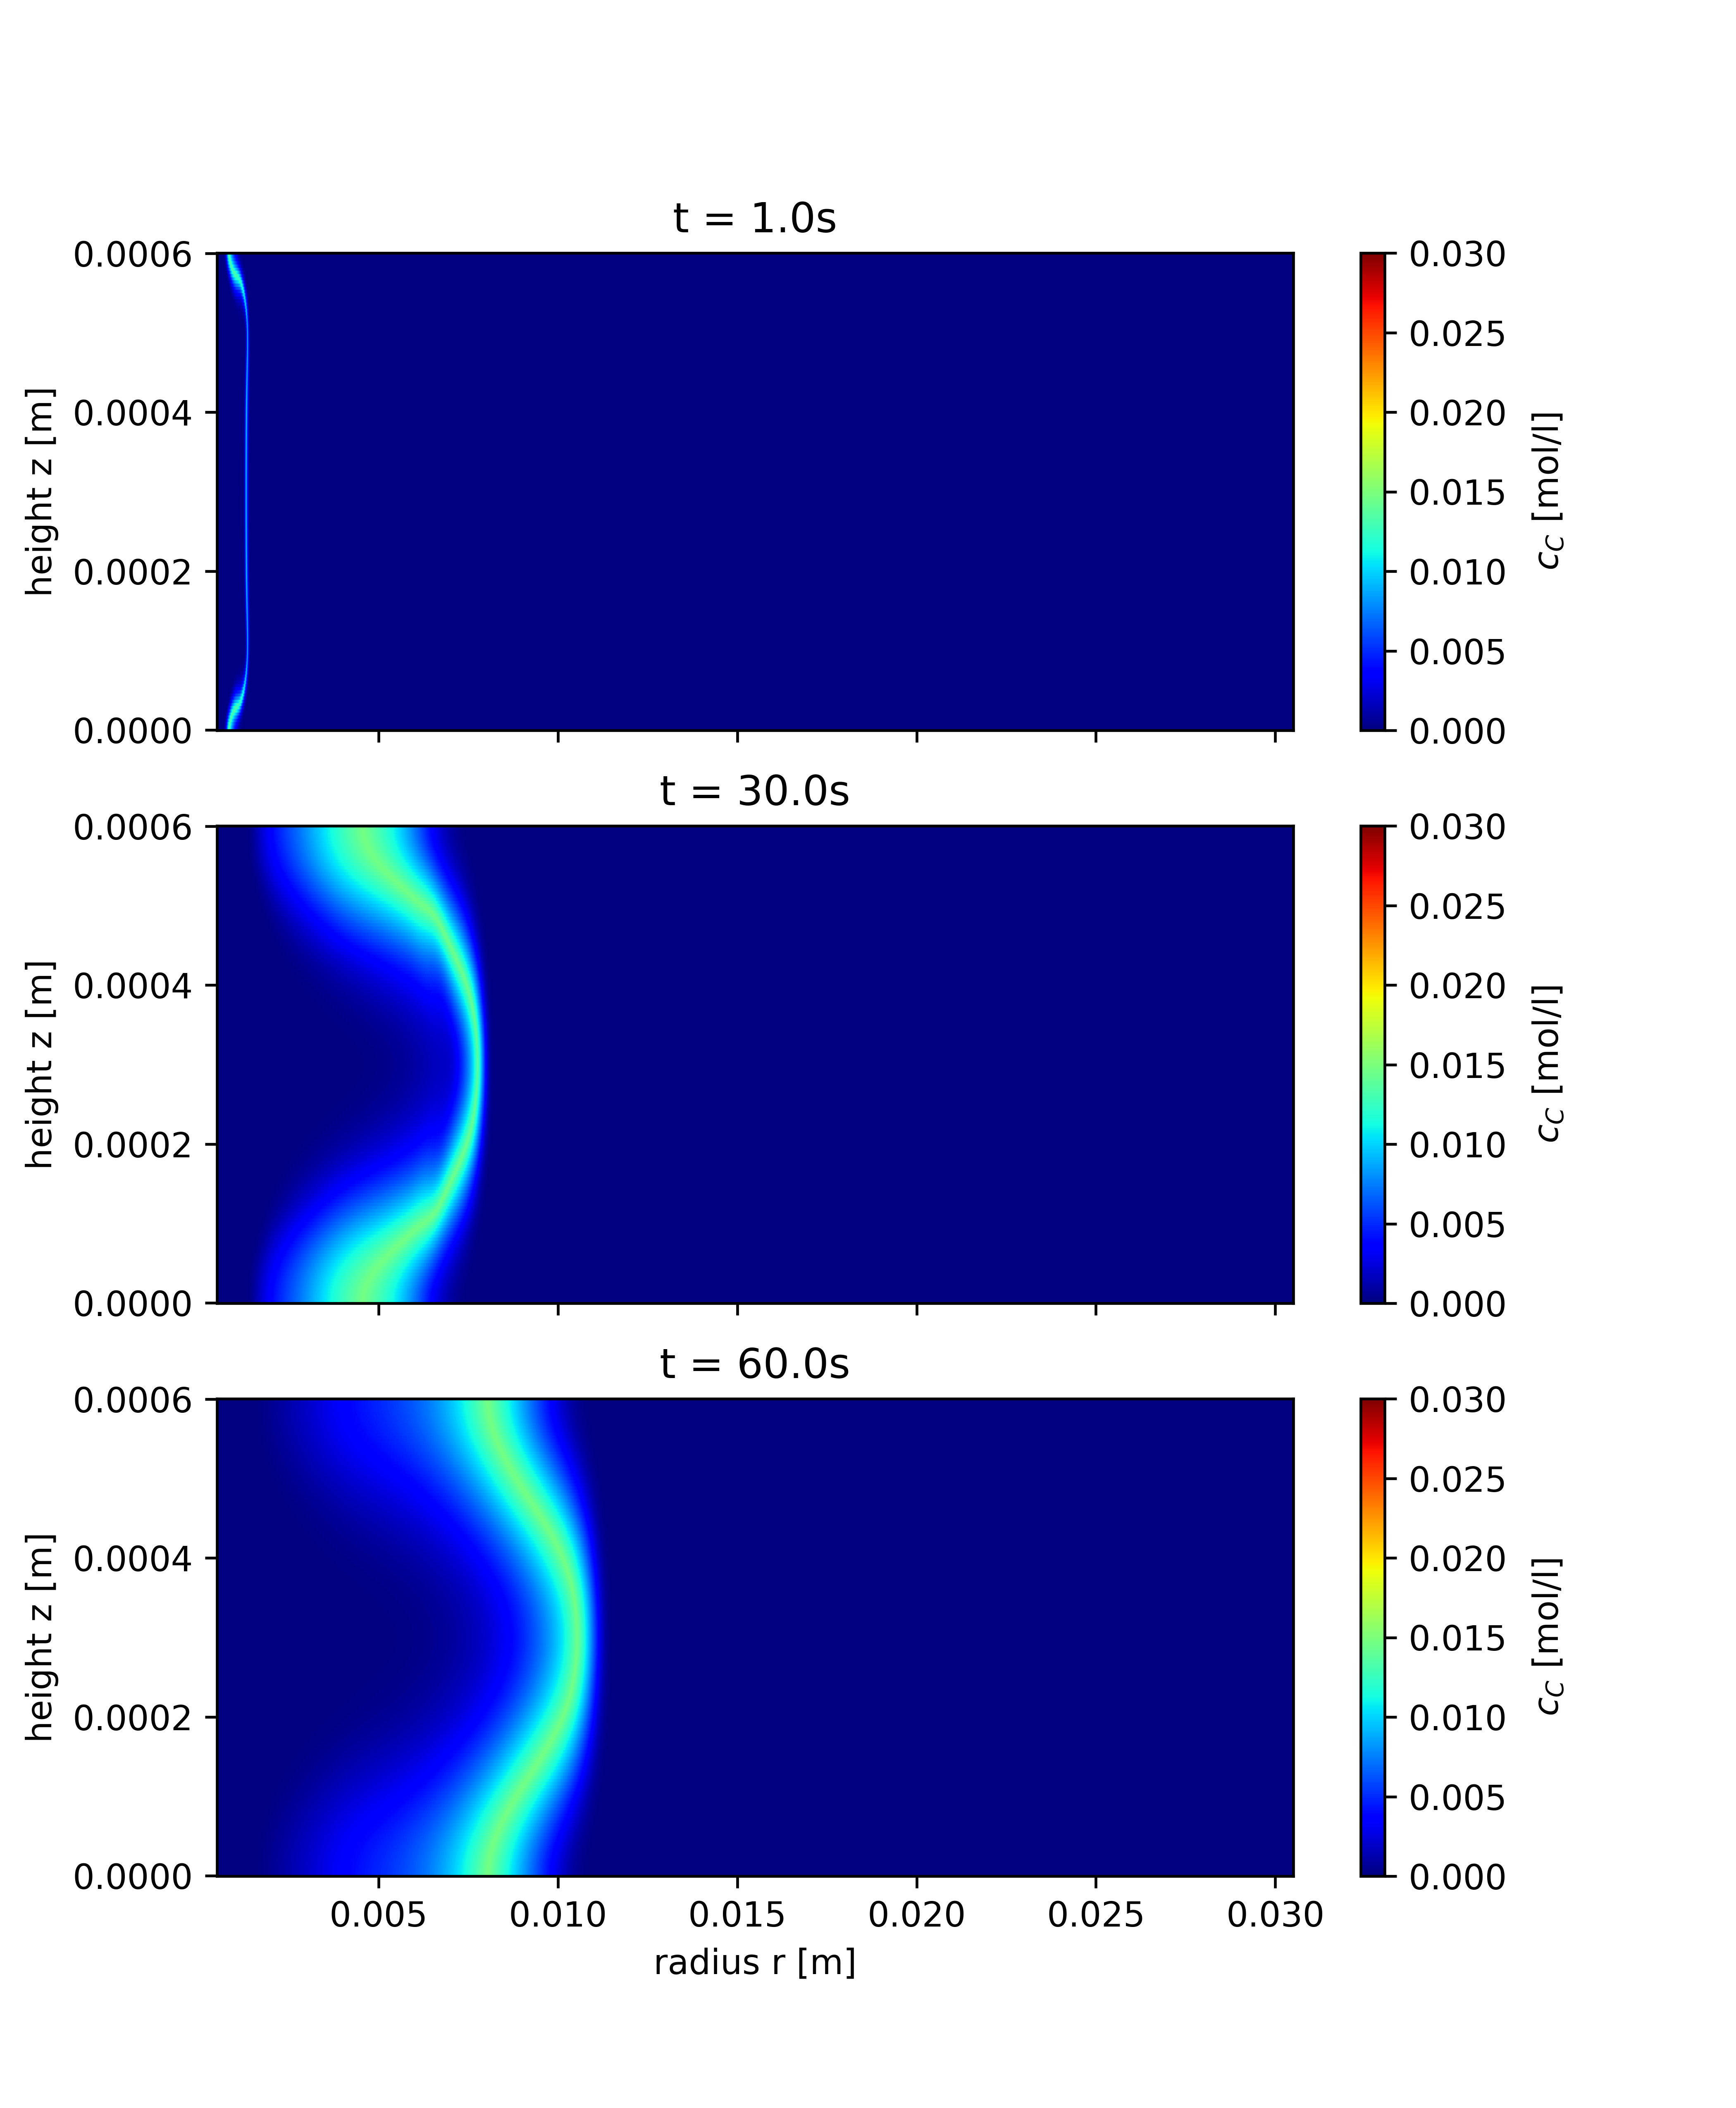
\includegraphics[angle=0, scale=0.41]{front_shape1} }}%
	\qquad
	\subfloat[\centering front shape for h0.2mm Pe2050 Sc2430]{{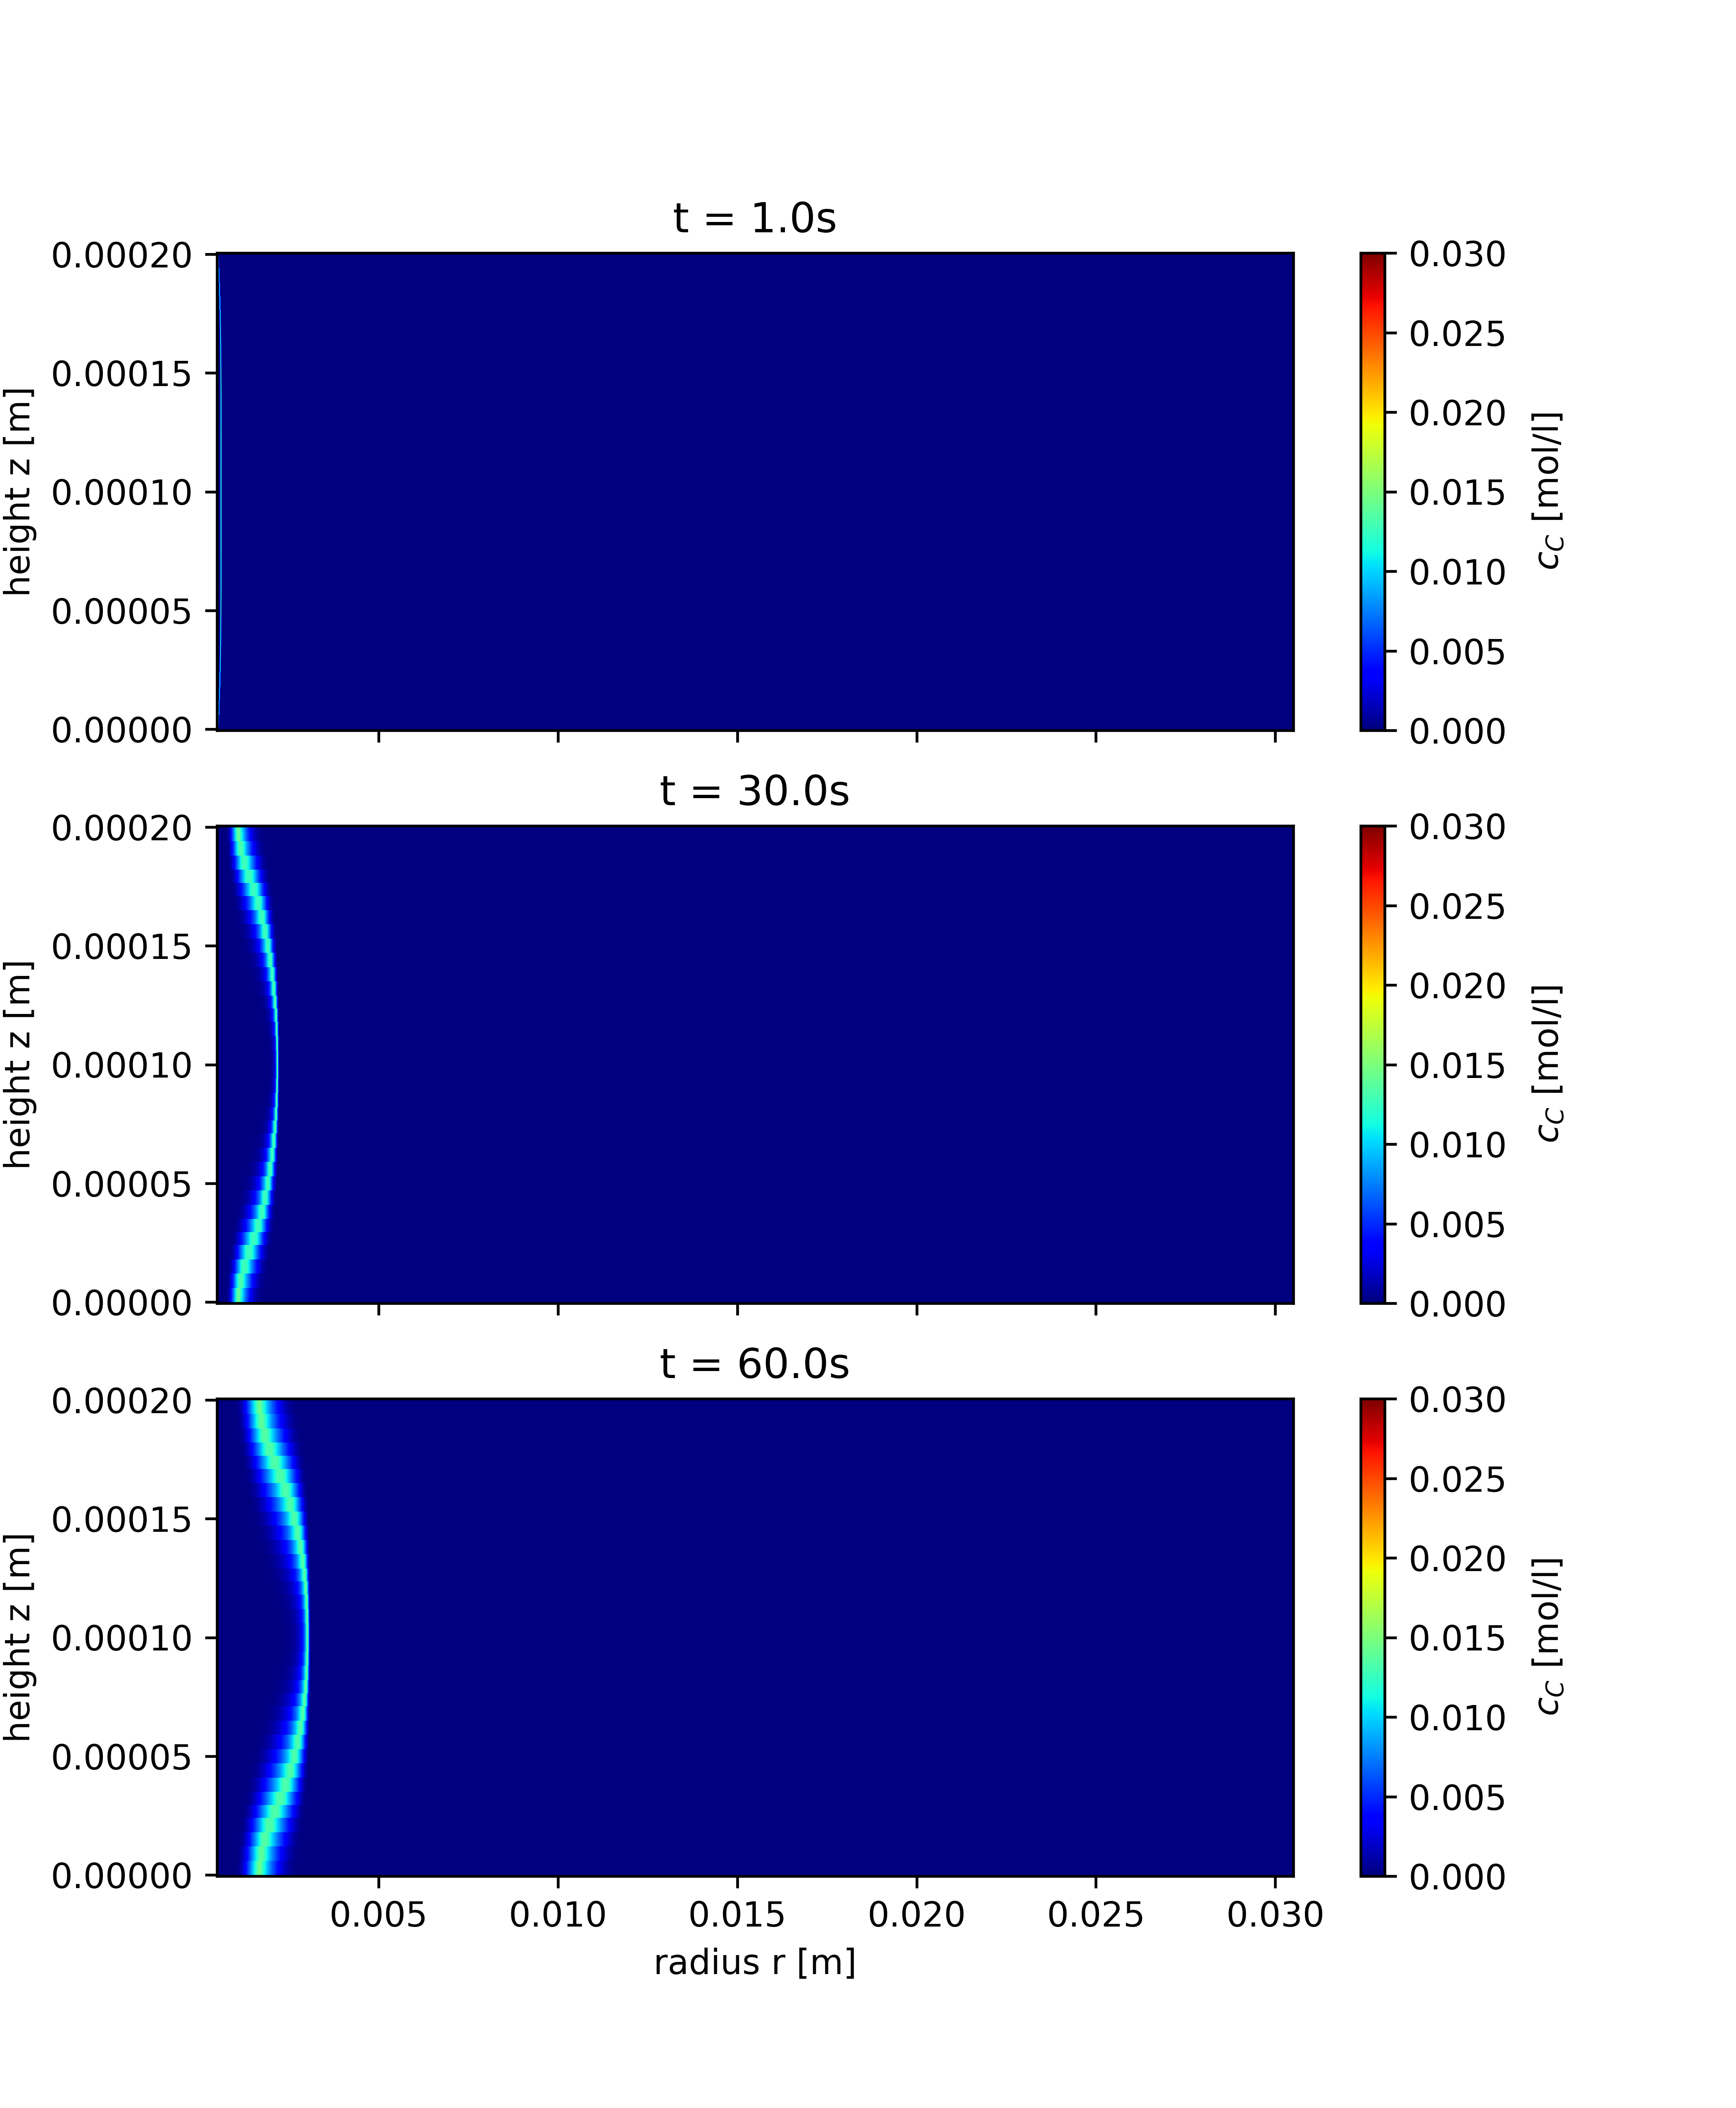
\includegraphics[angle=0, scale=0.41]{front_shape2} }}%
	\caption{example front shapes}%
	\label{fig: shape_examp}%
\end{figure}

\section{front positions}

The front positions behave in a similar way for all 3 reactor geometries. So in \autoref{fig: front_pos_h2_SC12E4} and \autoref{fig: front_pos_h2_SC243E3} the positions for each Schmidt-Number are shown
for the geometry containing a gap height of 0.2mm.
% two figures on same page
\begin{figure}[htbp]
	\centering
	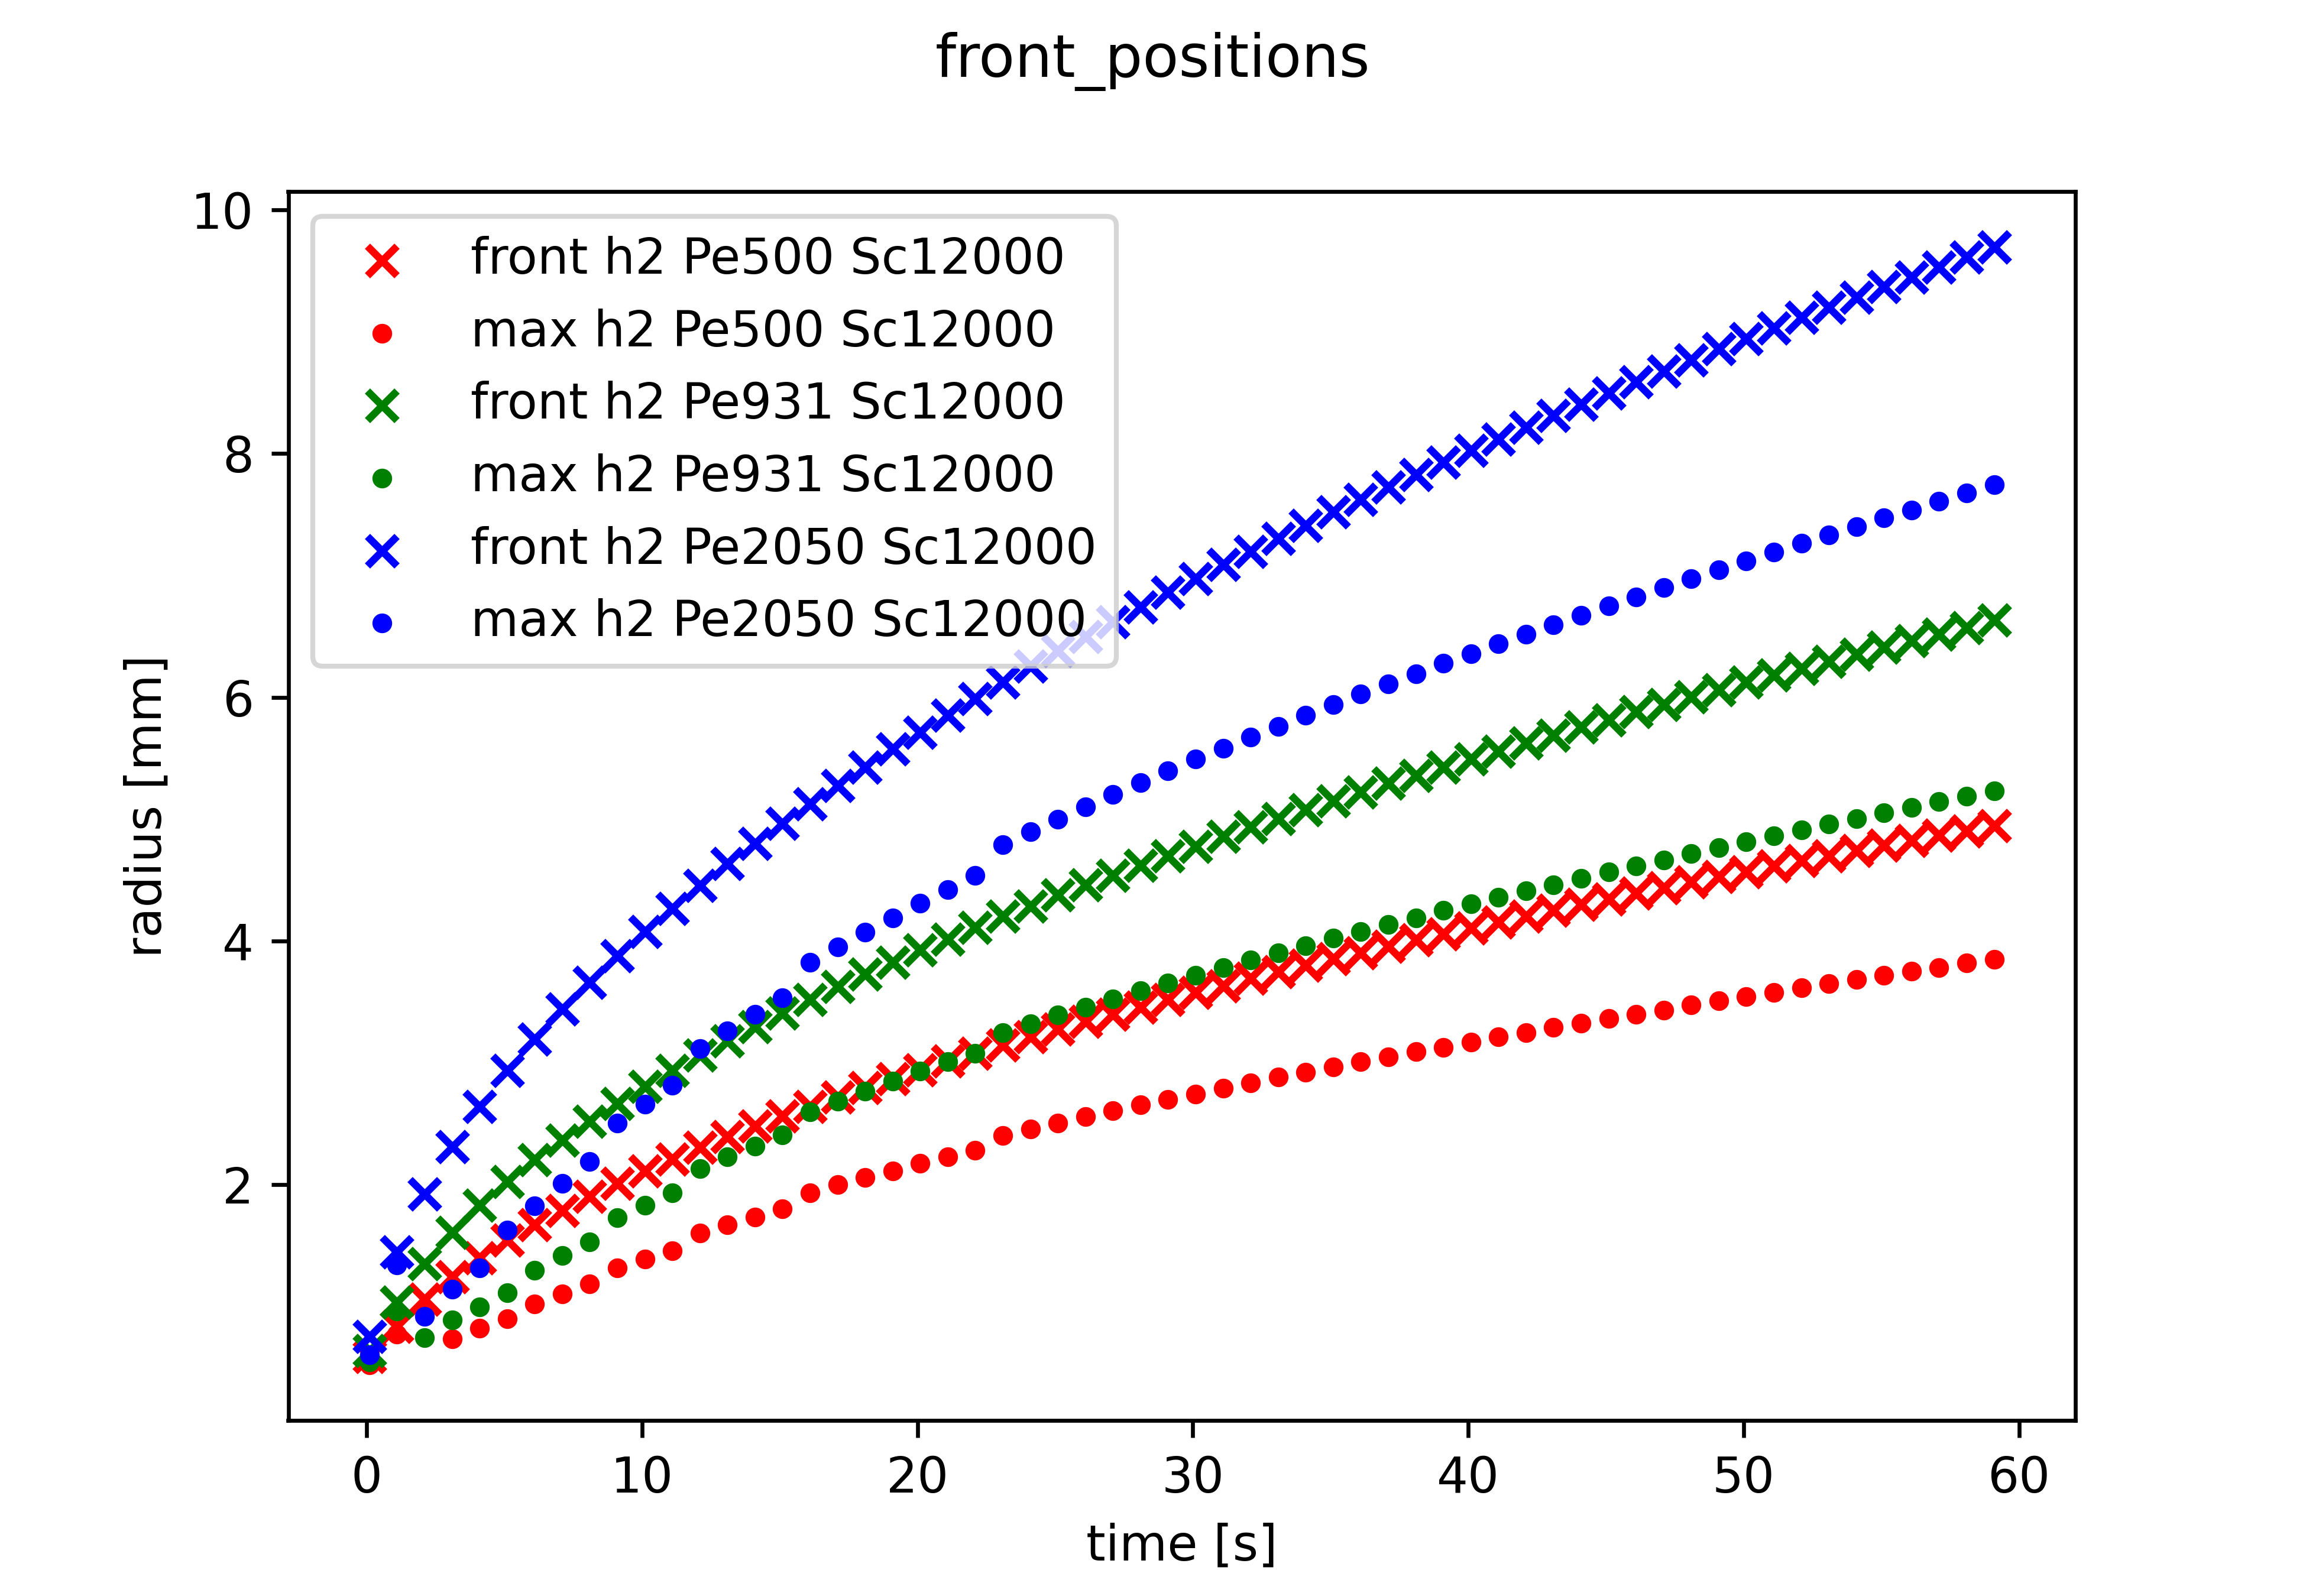
\includegraphics[width=.9\linewidth]{front_pos_h2_SC12E4}
	\caption{positions for h 0.2mm Sc 12000\label{fig: front_pos_h2_SC12E4}}\bigskip
	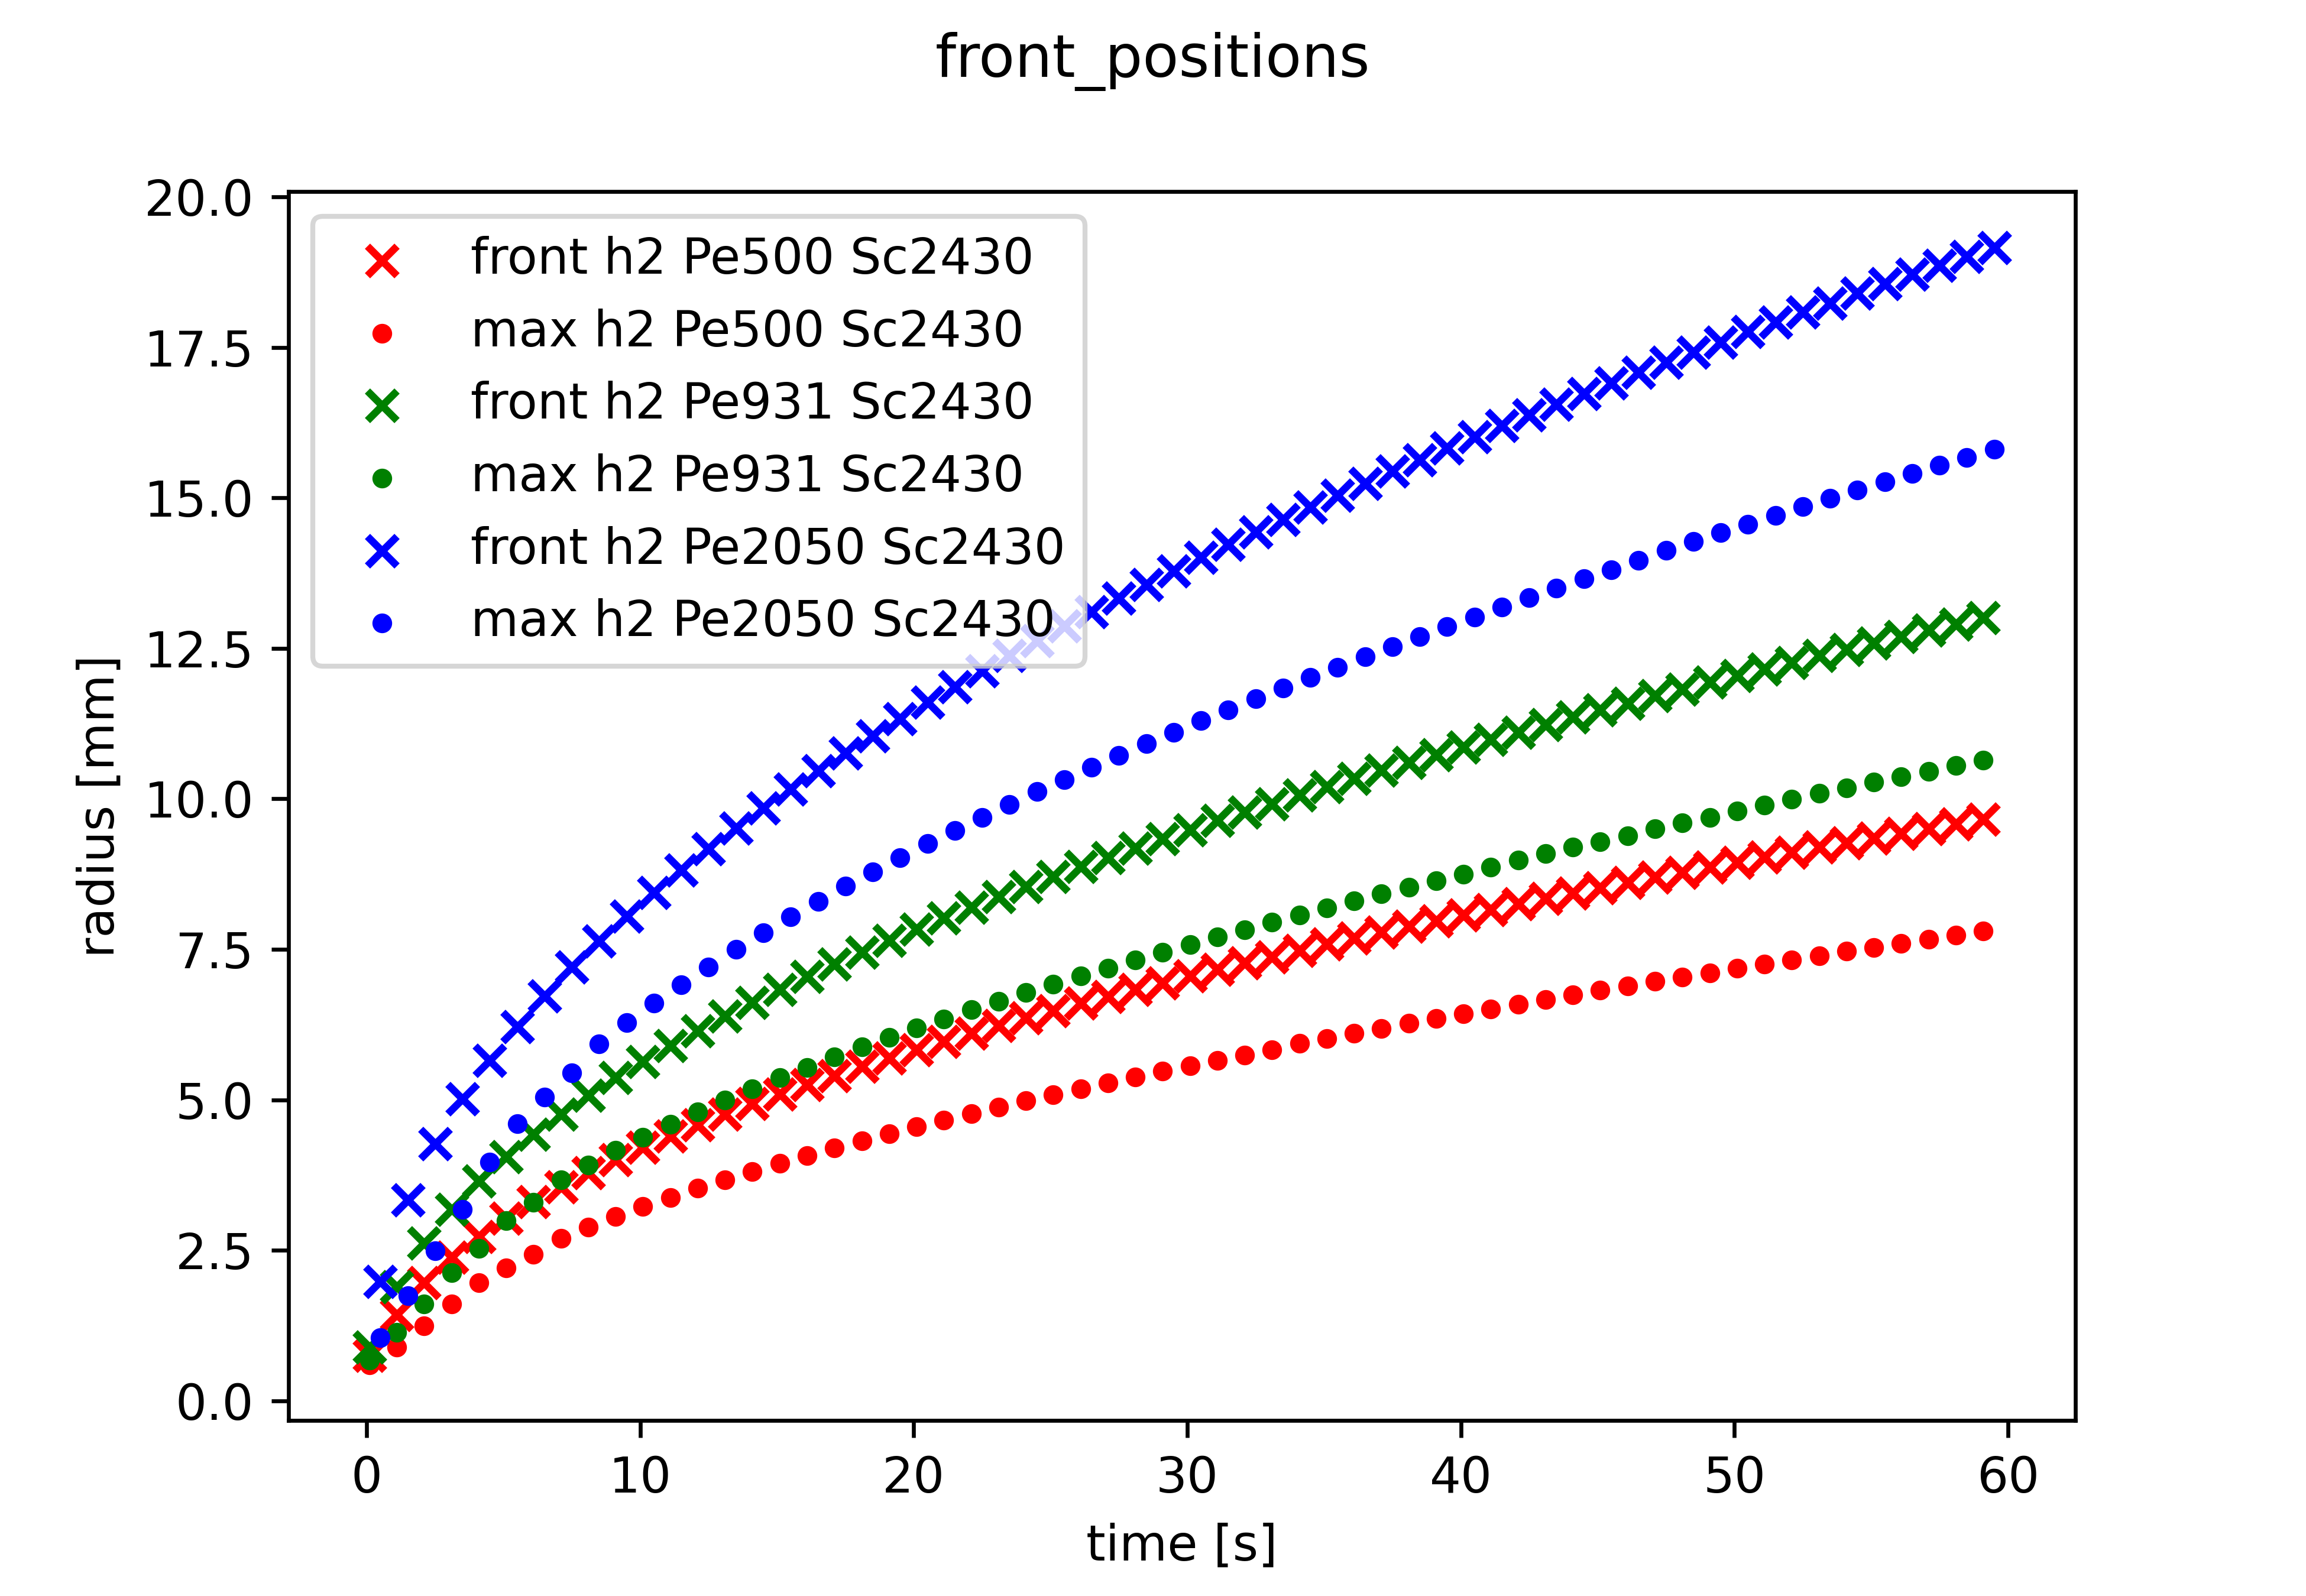
\includegraphics[width=.9\linewidth]{front_pos_h2_SC243E3}
	\caption{front positions for h 0.2mm Sc 2430\label{fig: front_pos_h2_SC243E3}}
\end{figure}

From these two graphs it can be seen that the front positions seem to follow a square root approach. The front and maximum travel faster for higher Peclet-Numbers, which can be explained by the different input velocities set. The maxima positions show similar behaviour to the front positions. With increasing input velocity the difference between the fronts front and maximum positions decreases. The decrease is more significant for cases with lower Peclet-Numbers. For these cases due to their lower inlet velocity the distance between the front and maximum is higher. A sleight change in input velocity has a large effect here seen when comparing plots for Peclet-Numbers 500 and 931.

When comparing the plots for Schmidt-Number 2430 with the one for a Schmidt-Number of 12000 it can be observed that all fronts travel nearly double the distance within the same time of 60 seconds. This can be explained mainly by the lower diffusion coefficient for the higher Schmidt-Number case. The diffusion coefficient for the lower Schmidt-Number case is $4 \text{.}11 \cdot 10^{-10} \left[ \frac{\mathrm{m^2}}{\mathrm{s}} \right]$ and the one for the higher case is $1\text{.}0 \cdot 10^{-10} \left[ \frac{\mathrm{m^2}}{\mathrm{s}} \right]$.
Since the velocity magnitude decreases very quickly for a axisymmetric reactor (see \autoref{fig: field_example}) diffusion plays a more and more significant role while the front travels through the reactor.
\section{front widths}

\section{formed product}

\end{document}